%\documentclass[letterpaper]{article}
\documentclass[12pt]{article}

\usepackage[letterpaper, portrait, margin=1in]{geometry}

\usepackage{array}	% for \newcolumntype macro
\usepackage{caption}
\usepackage{graphicx}    % This package is used for Figures
\usepackage{rotating}           % This package is used for landscape mode.
\usepackage{epsfig}
\usepackage{comment}
\usepackage{url}
\usepackage{amsmath}
\usepackage{amssymb}
\usepackage{cite}
\usepackage{float}
\usepackage{hyperref}
\usepackage{subfig}
\usepackage{amsmath}
\usepackage{multirow}
\usepackage[T1]{fontenc}
\usepackage[all]{nowidow}
\usepackage[table]{xcolor}
\usepackage{siunitx}
\usepackage{listings}
\usepackage{notoccite}
\usepackage{grffile} % can use example.0.1.png
\usepackage{tabularx}		% Fill to margin on tables, control table width
\usepackage[normalem]{ulem}			% for strike through \sout{}
\usepackage{anyfontsize} % for the GIMP large letters
\usepackage{listings} % color the code
\usepackage{color} % to define colors
\usepackage{hhline} % to manually insert a vertical line with | or #
\usepackage{multicol} % Multiple columns
\usepackage{pgfplots} % Plotting in LaTeX
\usepackage{enumitem} % Globally change enumerate settings. Also allows for alpha/roman switch.
\setlist{nosep} % or \setlist{noitemsep} to leave space around whole list
\usetikzlibrary{arrows} % For triangular-headded arrows
\usetikzlibrary{patterns} % for patterns
\usepackage[thinlines]{easytable} % For simpler table commands

\newcommand{\degrees}{$^\circ$}
\newcolumntype{M}{>{\vspace*{1cm}\hfill}p{0.223\textwidth}<{\hfill\vspace*{1cm}}} % Middle aligned

\usepackage{fancyhdr} % To create headers
\pagestyle{fancy}
\rhead{Dr. Kunz}
\newcommand{\docTitle}{Equipotential Lines}
\chead{PHYS 2150 \docTitle}
\begin{document}
\section*{Theory}
In class, we learned about electric potential energy. For simple point charges, this energy is proportional to $1/r$. However, for more complicated systems (such as two charged plates), the electric potential energy dependence is less obvious. Fortunately, it is still possible to ``map out'' the electric potential energy with equipotential lines. 

Equipotential lines are lines where the potential energy is the same. Figure~\ref{fig:equipotential} shows equipotential lines in purple and electric field lines in black. Here, any point on a given circle has the same potential energy since it's the same distance from the positive charge.

\begin{figure}[!h]
\begin{center}
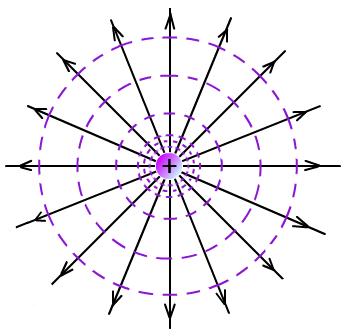
\includegraphics[width=0.5\textwidth]{equipotential}
\caption{Schematic of a point charge. The solid black lines are the electric field lines. The purple dashed lines are the equipotential lines.}
\label{fig:equipotential}
\end{center}
\end{figure}

In this lab, we'll be measuring voltage. Voltage is related to electric potential energy as
\[
V = \frac{E_{electric}}{q}=\frac{kq}{r}
\]

The units of volts, then, are
\[
1\text{ V} = 1\text{ N}\cdot\text{m}/\text{C}
\]

\section*{Experiment}
In this lab, we'll be mapping out the equipotential lines for several configurations.
\begin{enumerate}
	\item{Choose a configuration board (see Figure~\ref{fig:config_board}). This board may be in the front or back of the classroom.}
	\item{Copy the schematic onto a separate sheet of paper. Your instructor should teach you how to do this accurately.}
	\item{Turn the mapping board over (see Figure~\ref{fig:mapping_board}). Screw the configuration board into the bottom of the mapping board.}
	\item{Turn the mapping board right-side-up.}
	\item{Using either tape or the legs of the mapping board, fix the schematic onto the top of the mapping board.}
	\item{In your notes, sketch a prediction of what both the electric field lines and equipotential lines will look like.}
	\item{Turn your multimeter to measure voltage (DC).}
	\item{Use the probe to measure the voltage on the mapping board. Your instructor should teach you how to operate the multimeter and the probe if you do not know how.}
	\item{Select a voltage (around 3 V is a good start). Mark the spot where you measured the voltage with a pencil, like in Figure~\ref{fig:pencil}. Keep probing for this voltage and marking the spot until you have enough points to form a curve (at least five points).\label{itm:voltselect_loop_start}}
	\item{Once you have at least five points on your equipotential curve, connect the points. Remember to write down what voltage you measured next to the curve.\label{itm:voltselect_loop_end}}
	\item{Repeat steps~\ref{itm:voltselect_loop_start}--\ref{itm:voltselect_loop_end} until you have at least five different equipotential curves.}
	\item{Repeat the entire process for one additional configuration. Just like with all labs, \textbf{you should rotate responsibilities!}}
\end{enumerate}

\begin{figure}[!h]
	\begin{center}
		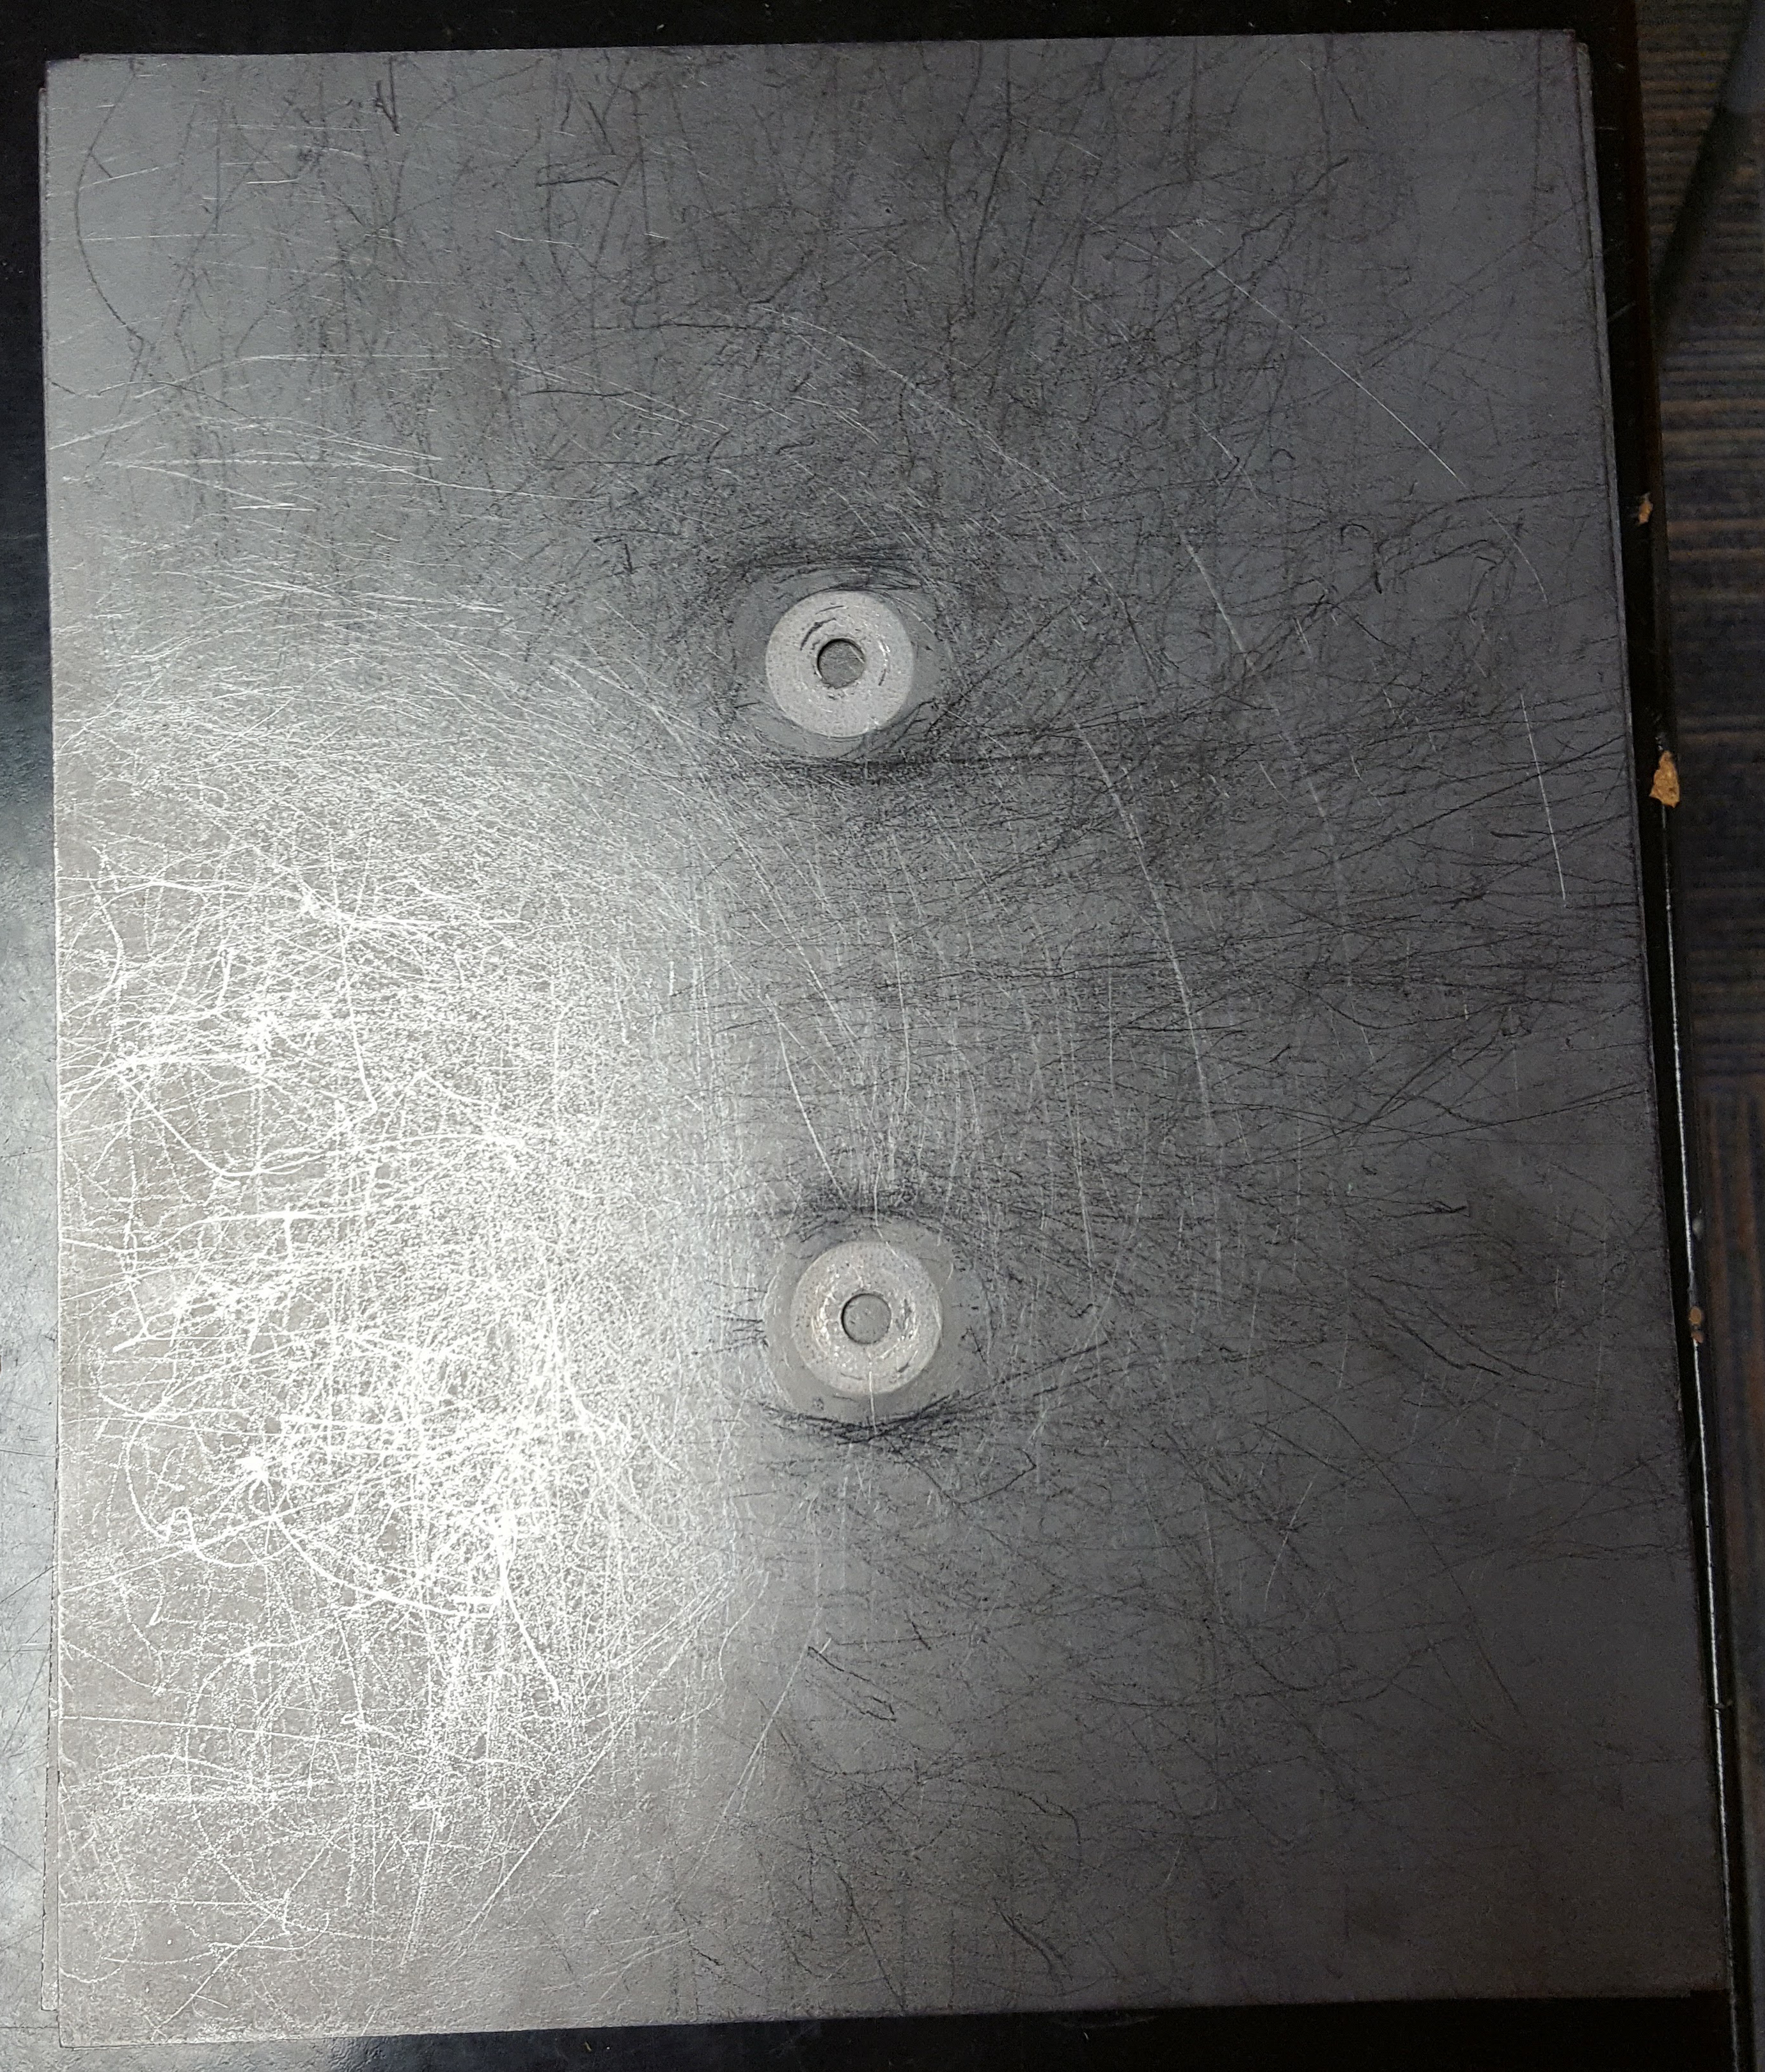
\includegraphics[width=0.5\textwidth]{config_board}
		\caption{An example of a configuration board.}
		\label{fig:config_board}
	\end{center}
\end{figure}

\begin{figure}[H]
	\begin{center}
		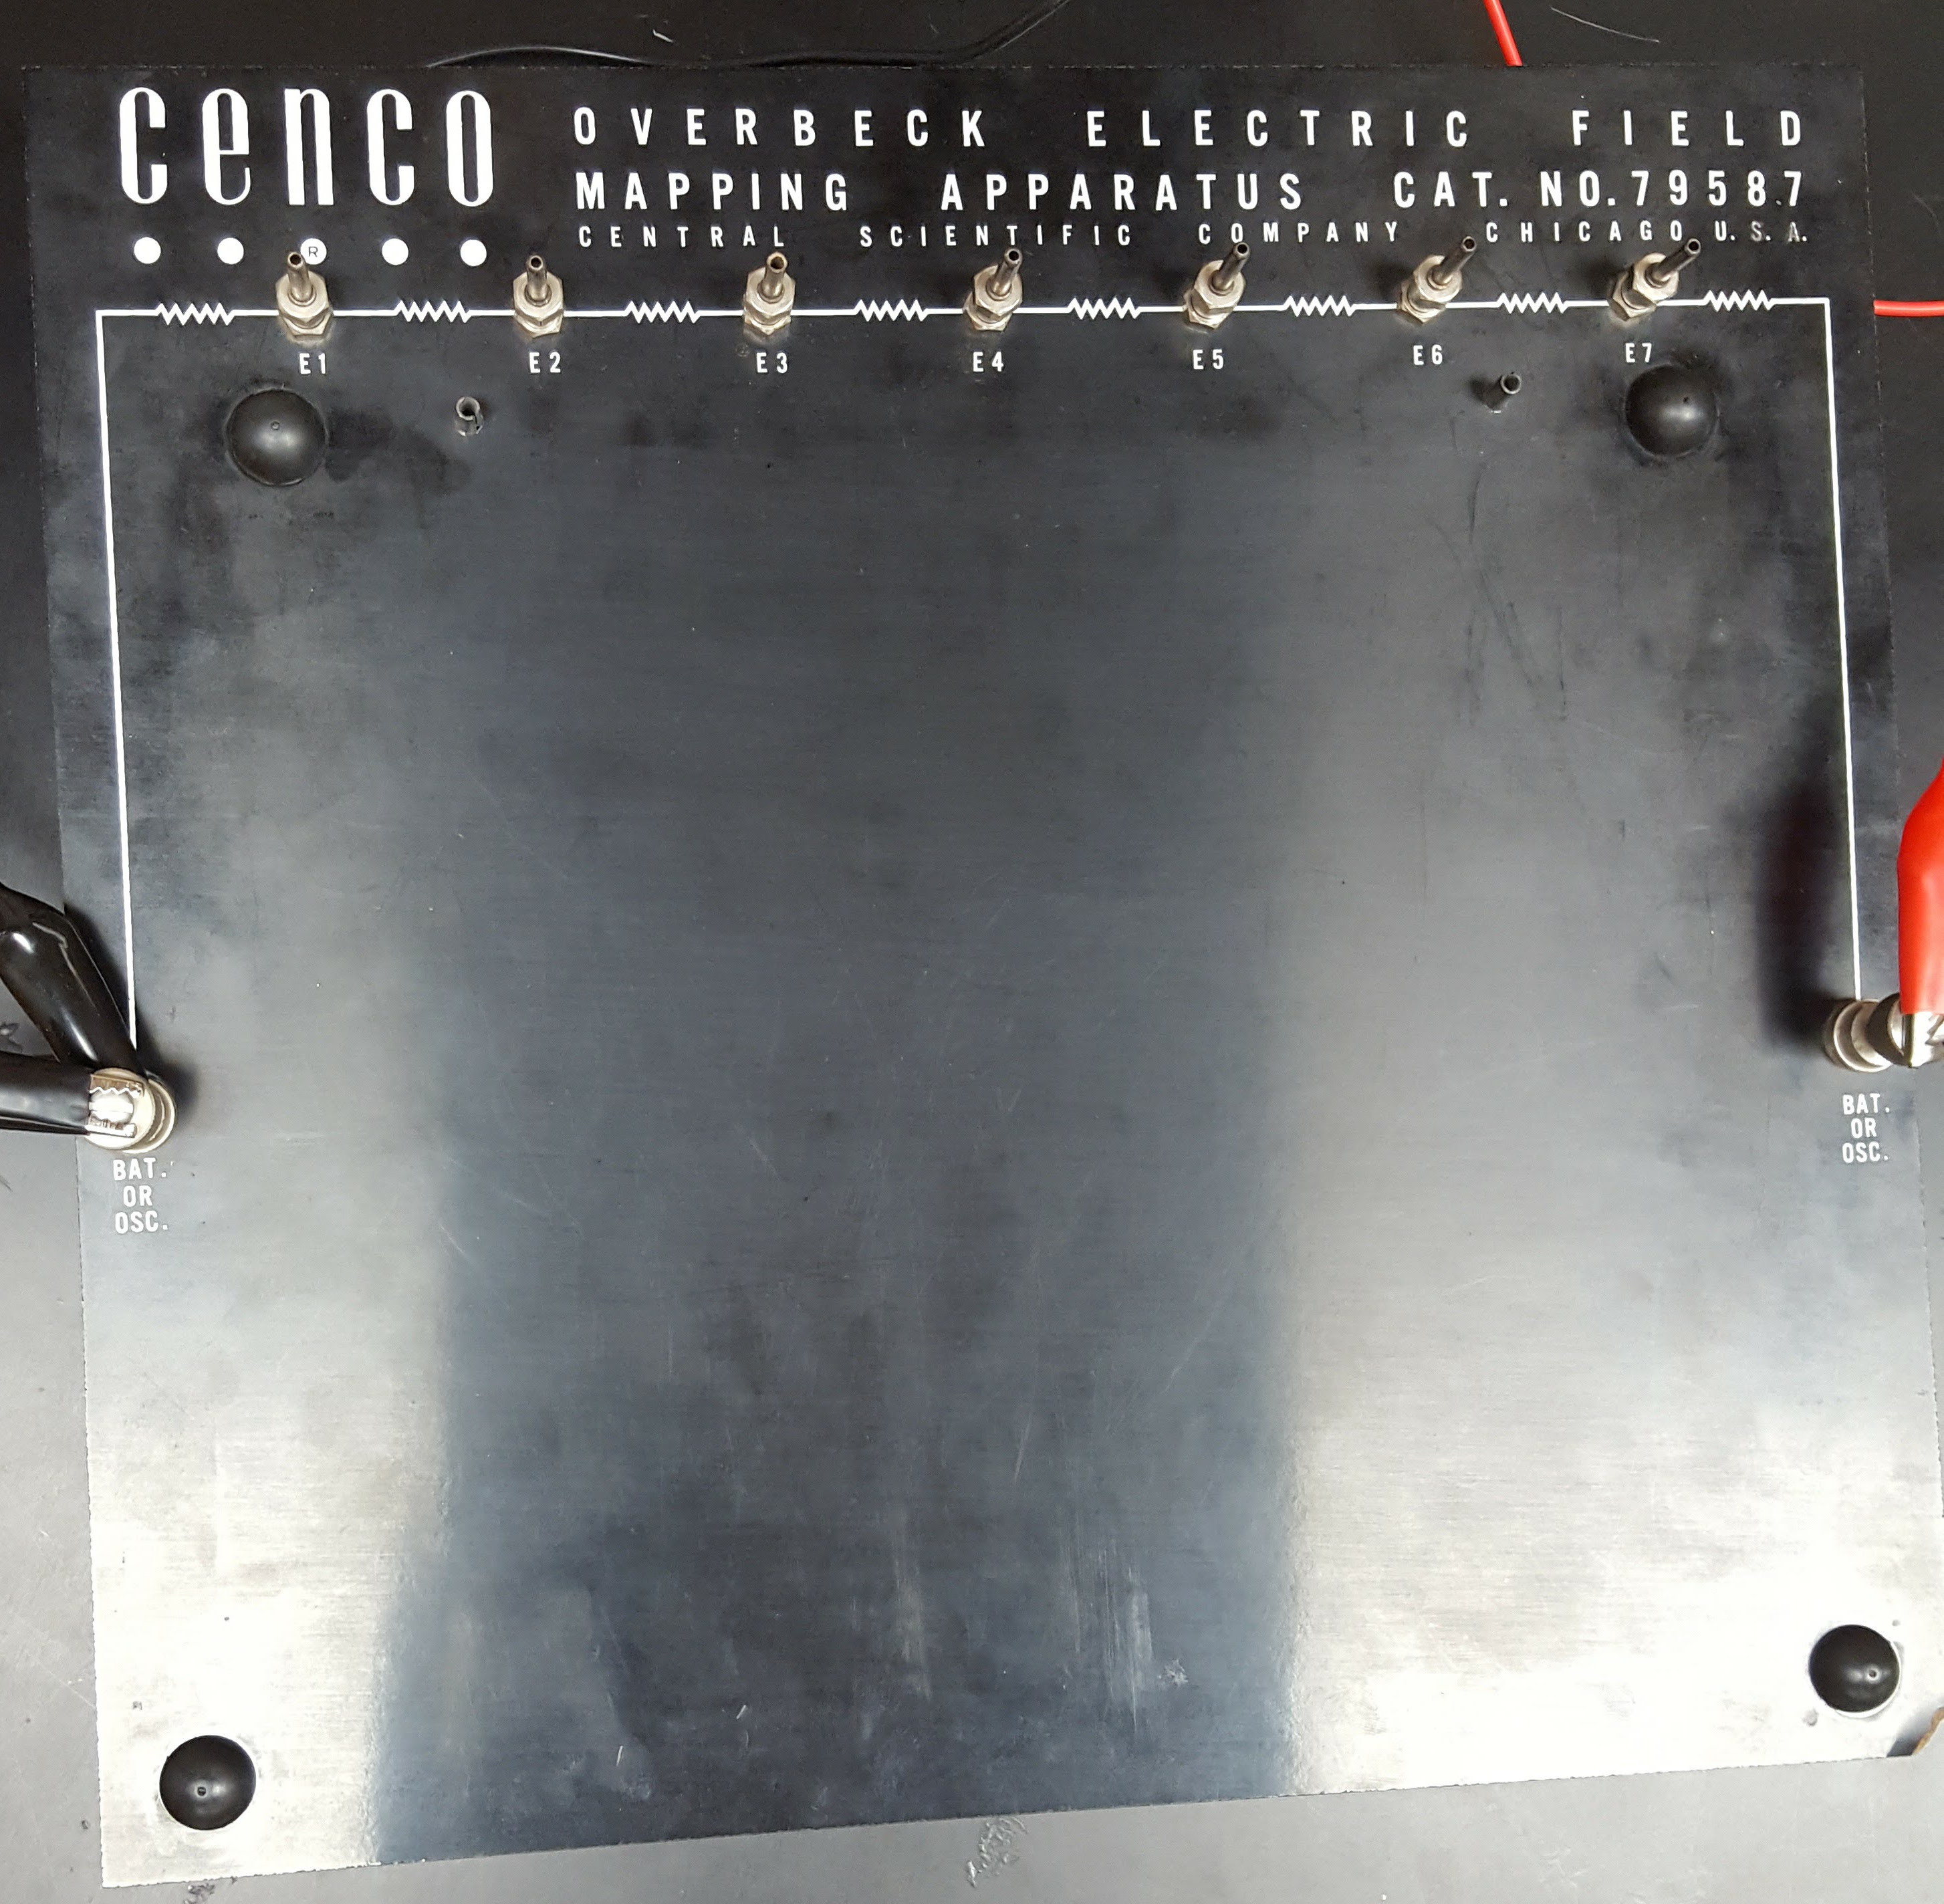
\includegraphics[width=0.5\textwidth]{mapping_board}
		\caption{The a mapping board.}
		\label{fig:mapping_board}
	\end{center}
\end{figure}

\begin{figure}[H]
	\begin{center}
		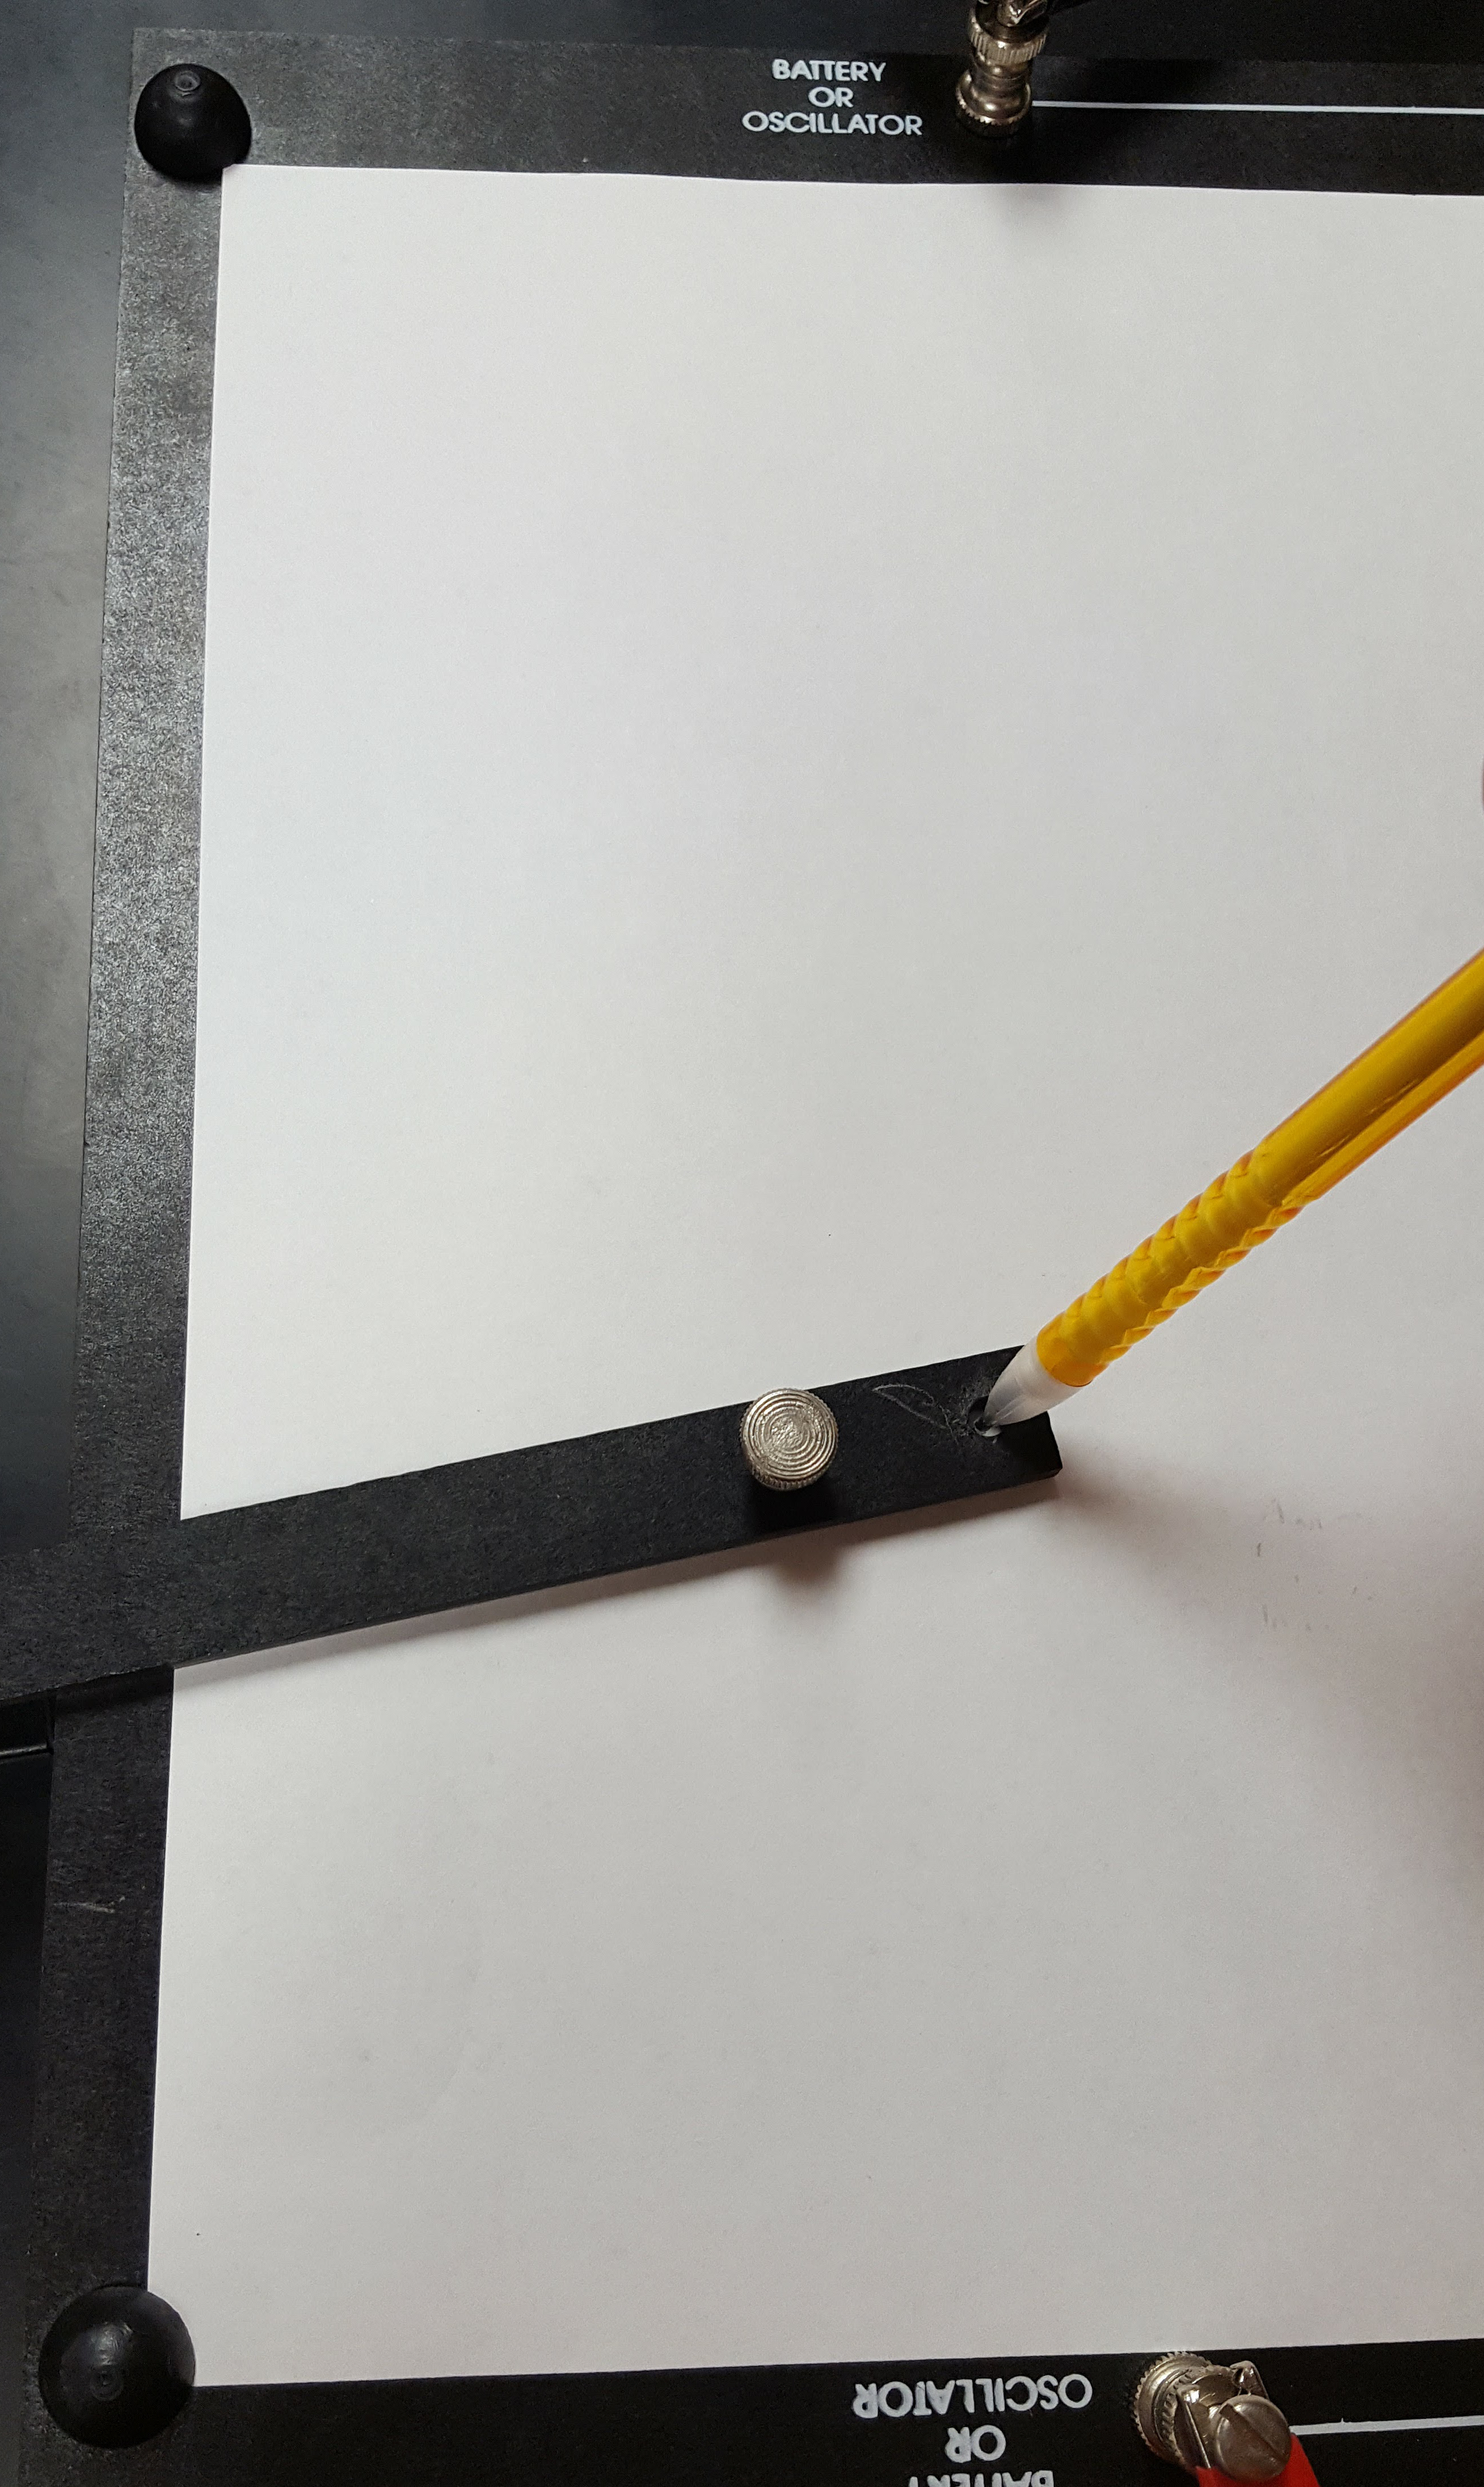
\includegraphics[width=0.25\textwidth]{pencil}
		\caption{How to mark on the paper with a pencil. Note that the pencil is in the hole.}
		\label{fig:pencil}
	\end{center}
\end{figure}

\section*{Questions}
\begin{enumerate}
	\item{List at least three possible errors that you encountered during this lab.}
	\item{Did your predictions match the experimental results? How were they different?}
\end{enumerate}

\end{document}

